\begin{enumerate}[label=\thesection.\arabic*.,ref=\thesection.\theenumi]
\numberwithin{equation}{enumi}
\item Find the range of k such that given characteristic equation
\begin{align}
s(s^3+2s^2+s+1) +k(s^2+s+1) = 0
\label{eq:ee18btech11042_1}
\end{align}
is stable.

\solution
The General form of characteristic equation :
\begin{align}
1+G(s)H(s) = 0
\label{eq:ee18btech11042_2}    
\end{align}
\center 
    For a system to be marginally stable , nyquist plot passes through (-1,0 ). Generally we will draw nyquist plot for open loop gain G(s)H(s).So,  1+G(s)H(s) passes through through (0,0)

\begin{align}
Real part = \omega^4 - \omega^2(k+1) +k = 0
\label{eq:ee18btech11042_3}
\end{align}
\begin{align}
Imaginary part = -\omega^3 +\omega(w+1) = 0
\label{eq:ee18btech11042_4}
\end{align}
By equating real and imaginary to 0 .We get,
\begin{align}
k = 0
\label{eq:ee18btech11042_5}
\end{align}
as minimum value system to be stable.
\item For a nyquist plot,no.of clock wise encirclement's around the point(-1,0) for a open loop transfer function gives the total no. right hand side  zeros ,
We can verify it through nyquist plot

\begin{figure}[!h]
  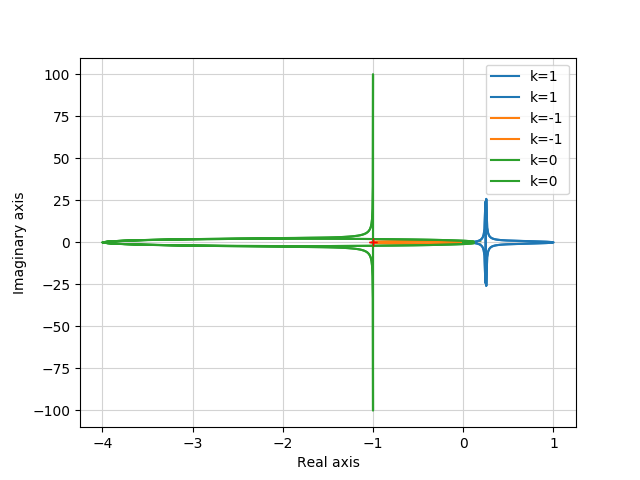
\includegraphics[width=\columnwidth]{ee18btech11042_1.png}
  \label{fig:ee18btech11042_1.png}
\end{figure}


\center The following python code generates the nyquist plot : 
\begin{lstlisting}
codes/ee18btech11042_1.py
\end{lstlisting}
\item Verifying k value using Routh-hurwitz criterion
Characteristic equation(polynomial):
\begin{align}
s^4+2s^3+s^2(k+1)+s(k+1)+k = 0
\label{eq:ee18btech11042_6}
\end{align}
\mydet{s^4\\s^3\\s^2\\s^1\\s^0}
\mydet{1 & k+1 & k\\ 2 & k+1 & 0\\ \frac{k+1}{2} & k & 0\\ \frac{(k-1)^2}{2} & 0 & 0 \\ k & 0 & 0}
From this we can say for system to be stable,all values of determinant should be greater than 0.So,minimum value of k is,
\begin{align}
 k = 0
\label{eq:ee18btech11042_7}
\end{align}
The range of k system to be stable
\begin{align}
0<k<\infty
\label{eq:ee18btech11042_8}
\end{align}
\item We can verify it through following python code
\begin{lstlisting}
codes/ee18btech11042_2.py
\end{lstlisting}
\end{enumerate}